\documentclass[conference]{IEEEtran}
\IEEEoverridecommandlockouts
\usepackage{cite}
\usepackage{amsmath,amssymb,amsfonts}
\usepackage{algorithm}
\usepackage{algorithmic}
\usepackage{graphicx}
\usepackage{textcomp}
\usepackage{xcolor}
\usepackage{tikz}
\usepackage{booktabs}
\usetikzlibrary{shapes.geometric, shapes.symbols, arrows.meta, positioning, fit, backgrounds, calc}

\def\BibTeX{{\rm B\kern-.05em{\sc i\kern-.025em b}\kern-.08em
    T\kern-.1667em\lower.7ex\hbox{E}\kern-.125emX}}

\begin{document}

\title{Class-Aware Reputation Defense and Sub-Cluster Collusion Mitigation for Byzantine-Robust Federated Intrusion Detection}

\author{
\IEEEauthorblockN{Pratham Mourya, Dhruv Shrivastava, Kritesh Goud}
\IEEEauthorblockA{
Department of Computer Engineering \\
School of Technology Management \& Engineering \\
Email: your-email@example.edu
}
}

\maketitle

\begin{abstract}
Federated Learning (FL) enables distributed organizations to collaboratively train an Intrusion Detection System (IDS) without exchanging raw telemetry, preserving privacy under regulations like GDPR and India's DPDP Act. However, conventional FL aggregation assumes honest participation, rendering models highly vulnerable to Byzantine poisoning, adaptive evasion, and coordinated multi-client collusion. In this paper, we present, implement, and empirically evaluate an adaptive, class-aware reputation defense with sub-cluster collusion mitigation for federated IDS. The system scores incoming model updates against a Byzantine-robust geometric-median reference using three complementary signals -- cosine directional alignment, variance-floor-bounded Median Absolute Deviation (MAD) magnitude scoring, and validation semantic impact -- augmented by a pairwise update correlation graph that detects tight collusion sub-clusters. Trust is tracked on a per-class basis via an Exponentially Weighted Moving Average (EWMA) $R(i, c)$ matrix, governing a three-tier participant state machine (\texttt{TRUSTED} $\to$ \texttt{PROBATION} $\to$ \texttt{QUARANTINED}) with automatic shadow recovery. Accepted updates are aggregated via a decoupled head/body rule that preserves shared feature representations while cutting off compromised class decision boundaries ($R < 0.50$). All state transitions are immutably committed to a SHA-256 permissioned audit ledger. We evaluate the architecture on the CICIoT2023 dataset under a Non-IID Dirichlet ($\alpha = 0.5$) partition across ten simulated organizations. Across a 4-attack benchmark (Targeted Label-Flip, Adaptive Norm-Clipping, Adaptive Cosine-Mimicry, and Coordinated Collusion), our defense consistently outperforms FedAvg, Multi-Krum, Trimmed Mean, and Coordinate Median, achieving 80.75\% test accuracy, 46.12\% macro-F1, and restoring target-class F1 from 19.77\% to 50.37\% with only 350.38~ms of per-round security overhead.
\end{abstract}

\begin{IEEEkeywords}
Federated Learning, Intrusion Detection System, Blockchain Audit Trail, Collusion Detection, Byzantine Robustness, Non-IID Dirichlet, CICIoT2023
\end{IEEEkeywords}

% ============================================================
\section{Introduction}
% ============================================================
AI-driven Intrusion Detection Systems (IDS) are essential for defending modern enterprise networks against malware, DDoS, botnets, and reconnaissance probes. Machine learning models require diverse cross-organizational telemetry, yet regulatory frameworks (GDPR, HIPAA, India's DPDP Act) prohibit sharing raw network logs. Federated Learning (FL) resolves this dilemma by decentralizing training: organizations train local models and share only gradient/weight updates ($\Delta w_i$) with a central coordinator.

Despite these privacy advantages, standard FL protocols (e.g., FedAvg) operate under an implicit trust model. Adversaries can submit poisoned weights to degrade global accuracy or embed backdoors that allow specific attack traffic to evade detection. This vulnerability is compounded by three real-world challenges:
\begin{enumerate}
    \item \textbf{Non-IID Skew}: Organizations observe heterogeneous traffic distributions; naive distance filters mistake legitimate statistical variance for adversarial poisoning.
    \item \textbf{Coarse Trust Granularity}: Traditional defenses treat trust as a single client-level scalar, discarding useful gradients across unaffected attack classes when a client is partially compromised.
    \item \textbf{Coordinated Collusion}: Sophisticated adversaries coordinate updates to mimic consensus directions, bypassing single-update anomaly checks.
\end{enumerate}

To overcome these limitations, we design and implement a class-aware reputation defense that validates updates against a geometric-median reference, isolates compromised classes through decoupled head/body aggregation, detects coordinated multi-client collusion via pairwise correlation graphs, and guarantees cryptographic auditability on a permissioned SHA-256 ledger.

% ============================================================
\section{Related Work}
% ============================================================
Recent literature has explored securing federated IDS through reputation and blockchain mechanisms:
\begin{itemize}
    \item \textbf{Reputation-Based FL}: Kang \emph{et al.}~\cite{kang2020reputation} introduced worker selection via reputation metrics. Rashid \emph{et al.} (TFFL)~\cite{rashid2025tffl} applied Subjective Logic on MNIST/CIFAR benchmarks. However, both use a single scalar trust score, failing to isolate class-specific poisoning.
    \item \textbf{Blockchain-Assisted FL-IDS}: Begum \emph{et al.} (BFLIDS)~\cite{begum2024bflids} and Ali \emph{et al.} (FL-BCID)~\cite{ali2025flbcid} log anomaly scores on-chain, but rely on single-signal heuristics evaluated against simple arithmetic means.
    \item \textbf{Multi-Dimensional Defenses}: FLARE~\cite{flare2025}, RepuNet~\cite{repunet2025}, and P4P~\cite{p4p2026} investigate non-IID client drift, while BlockFedZTA~\cite{blockfedzta2026} and PenTiDef~\cite{pentidef2026} incorporate privacy and audit trails. However, none combine per-class trust decomposition with active multi-client collusion detection and tested off-chain tamper verification.
\end{itemize}

% ============================================================
\section{Proposed System Architecture}
% ============================================================

\begin{figure*}[t]
\centering
\resizebox{0.95\textwidth}{!}{%
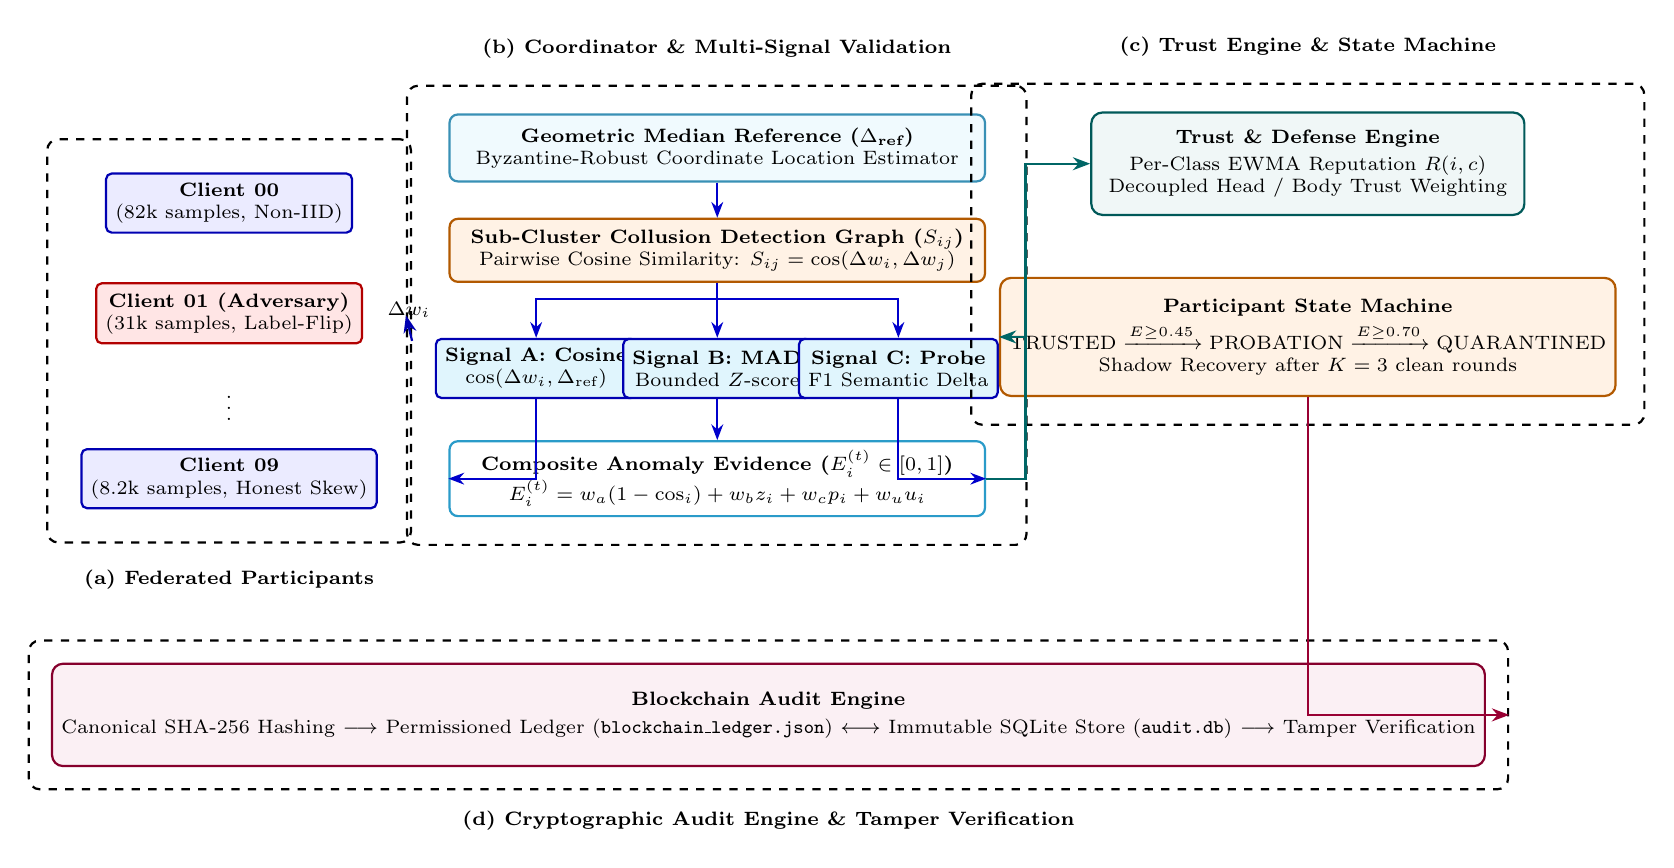
\begin{tikzpicture}[
    font=\small,
    chip/.style={rectangle, rounded corners=2pt, draw=blue!70!black, thick, fill=blue!8, minimum width=2.6cm, minimum height=0.75cm, align=center, font=\scriptsize},
    chipmal/.style={rectangle, rounded corners=2pt, draw=red!70!black, thick, fill=red!10, minimum width=2.6cm, minimum height=0.75cm, align=center, font=\scriptsize},
    bigbox/.style={rectangle, rounded corners=3pt, draw=cyan!70!black, thick, fill=cyan!6, align=center, font=\scriptsize},
    enginebox/.style={rectangle, rounded corners=4pt, draw=teal!70!black, thick, fill=teal!6, align=center, font=\scriptsize},
    auditbox/.style={rectangle, rounded corners=4pt, draw=purple!70!black, thick, fill=purple!6, align=center, font=\scriptsize},
    panel/.style={rectangle, rounded corners=4pt, draw, dashed, thick, inner sep=10pt},
    panellabel/.style={font=\scriptsize\bfseries, align=center},
    flow/.style={-{Stealth[length=2.2mm]}, thick},
    dataarrow/.style={-{Stealth[length=2mm]}, draw=blue!80!black, thick}
]

% Panel A: Participants
\node[chip] (cl0) at (1.8, 8.5) {\textbf{Client 00}\\(82k samples, Non-IID)};
\node[chipmal] (cl1) at (1.8, 7.1) {\textbf{Client 01 (Adversary)}\\(31k samples, Label-Flip)};
\node[font=\scriptsize] (dots) at (1.8, 6.0) {$\vdots$};
\node[chip] (cl9) at (1.8, 5.0) {\textbf{Client 09}\\(8.2k samples, Honest Skew)};

\node[panel, fit=(cl0)(cl1)(dots)(cl9), inner sep=12pt] (panelA) {};
\node[panellabel, below=6pt of panelA] {(a) Federated Participants};

% Panel B: Server Coordinator
\node[bigbox, minimum width=6.8cm, minimum height=0.85cm] (gm) at (8.0, 9.2) {
    \textbf{Geometric Median Reference ($\Delta_{\text{ref}}$)}\\
    Byzantine-Robust Coordinate Location Estimator
};

\node[bigbox, fill=orange!10, draw=orange!70!black, minimum width=6.8cm, minimum height=0.8cm] (coll) at (8.0, 7.9) {
    \textbf{Sub-Cluster Collusion Detection Graph ($S_{ij}$)}\\
    Pairwise Cosine Similarity: $S_{ij} = \cos(\Delta w_i, \Delta w_j)$
};

\node[chip, fill=cyan!12, minimum width=2.0cm] (sigA) at (5.7, 6.4) {\textbf{Signal A: Cosine}\\$\cos(\Delta w_i, \Delta_{\text{ref}})$};
\node[chip, fill=cyan!12, minimum width=2.0cm] (sigB) at (8.0, 6.4) {\textbf{Signal B: MAD}\\Bounded $Z$-score};
\node[chip, fill=cyan!12, minimum width=2.0cm] (sigC) at (10.3, 6.4) {\textbf{Signal C: Probe}\\F1 Semantic Delta};

\node[bigbox, fill=white, draw=cyan!80!black, minimum width=6.8cm, minimum height=0.65cm] (evidence) at (8.0, 5.0) {
    \textbf{Composite Anomaly Evidence ($E_i^{(t)} \in [0, 1]$)}\\
    $E_i^{(t)} = w_a(1-\cos_i) + w_b z_i + w_c p_i + w_u u_i$
};

\draw[dataarrow] (gm.south) -- (coll.north);
\draw[dataarrow] (coll.south) -- ++(0,-0.2) -| (sigA.north);
\draw[dataarrow] (coll.south) -- (sigB.north);
\draw[dataarrow] (coll.south) -- ++(0,-0.2) -| (sigC.north);
\draw[dataarrow] (sigA.south) |- (evidence.west);
\draw[dataarrow] (sigB.south) -- (evidence.north);
\draw[dataarrow] (sigC.south) |- (evidence.east);

\node[panel, fit=(gm)(coll)(sigA)(sigB)(sigC)(evidence), inner sep=10pt] (panelB) {};
\node[panellabel, above=6pt of panelB] {(b) Coordinator \& Multi-Signal Validation};

% Panel C: Trust Engine
\node[enginebox, minimum width=5.5cm, minimum height=1.3cm] (trusteng) at (15.5, 9.0) {
    \textbf{Trust \& Defense Engine}\\[2pt]
    Per-Class EWMA Reputation $R(i, c)$\\
    Decoupled Head / Body Trust Weighting
};

\node[enginebox, fill=orange!10, draw=orange!70!black, minimum width=5.5cm, minimum height=1.5cm] (statemach) at (15.5, 6.8) {
    \textbf{Participant State Machine}\\[2pt]
    $\text{TRUSTED} \xrightarrow{E \ge 0.45} \text{PROBATION} \xrightarrow{E \ge 0.70} \text{QUARANTINED}$\\
    $\text{Shadow Recovery after } K=3 \text{ clean rounds}$
};

\node[panel, fit=(trusteng)(statemach), inner sep=10pt] (panelC) {};
\node[panellabel, above=6pt of panelC] {(c) Trust Engine \& State Machine};

% Panel D: Audit
\node[auditbox, minimum width=15.5cm, minimum height=1.3cm] (auditeng) at (8.65, 2.0) {
    \textbf{Blockchain Audit Engine}\\[2pt]
    Canonical SHA-256 Hashing $\longrightarrow$ Permissioned Ledger (\texttt{blockchain\_ledger.json}) $\longleftrightarrow$ Immutable SQLite Store (\texttt{audit.db}) $\longrightarrow$ Tamper Verification
};

\node[panel, fit=(auditeng), inner sep=8pt] (panelD) {};
\node[panellabel, below=4pt of panelD] {(d) Cryptographic Audit Engine \& Tamper Verification};

% Connectors
\draw[flow, draw=blue!70!black] (panelA.east) -- node[above, font=\scriptsize] {$\Delta w_i$} (panelB.west);
\draw[flow, draw=teal!80!black] (evidence.east) -- ++(0.5,0) |- (trusteng.west);
\draw[flow, draw=teal!80!black] (evidence.east) -- ++(0.5,0) |- (statemach.west);
\draw[flow, draw=purple!80!black] (statemach.south) |- (panelD.east);

\end{tikzpicture}
}
\caption{System Architecture: (a) Federated clients; (b) Server Coordinator evaluating Multi-Signal Validator and Sub-Cluster Collusion Detector; (c) Trust \& Defense Engine governing per-class EWMA reputation and 3-tier state transitions; (d) Permissioned Blockchain Audit Engine.}
\label{fig:architecture}
\end{figure*}

\subsection{Multi-Signal Validation and Collusion Detection}
Each submitted update $\Delta w_i$ is validated against the geometric median reference $\Delta_{\text{ref}}$ via:
\begin{enumerate}
    \item \textbf{Directional Alignment ($\cos_i$)}: $\cos(\Delta w_i, \Delta_{\text{ref}})$.
    \item \textbf{Bounded MAD Z-Score ($z_i$)}: Evaluates update L2-norm against cohort median with a dynamic variance floor to protect honest non-IID variance.
    \item \textbf{Semantic Probing ($p_i$)}: Measures empirical macro-F1 delta on server validation data when candidate update is injected at $1/N$ step weight.
    \item \textbf{Sub-Cluster Collusion Penalty ($u_i$)}: Pairwise cosine similarity matrix $S_{ij} = \cos(\Delta w_i, \Delta w_j)$ is computed across all updates. Groups of clients with tight correlation ($S_{ij} > 0.88$) that simultaneously diverge from $\Delta_{\text{ref}}$ receive a progressive collusion penalty $u_i \in [0, 1]$.
\end{enumerate}

Composite evidence score $E_i^{(t)} \in [0, 1]$ is computed as:
\begin{equation}
E_i^{(t)} = w_a(1 - \cos_i) + w_b z_i + w_c p_i + w_u u_i,
\label{eq:evidence}
\end{equation}
with $w_a + w_b + w_c + w_u = 1$.

\subsection{Per-Class Reputation and State Transitions}
For every observed attack class $c$, reputation $R(i, c)$ adapts via an asymmetric EWMA:
\begin{equation}
R^{(t)}(i, c) = \beta \cdot R^{(t-1)}(i, c) + (1 - \beta) \cdot (1 - E_i^{(t)}).
\label{eq:reputation_update}
\end{equation}
Accumulated evidence governs state transitions: $\text{TRUSTED} \xrightarrow{E \ge 0.45} \text{PROBATION} \xrightarrow{E \ge 0.70} \text{QUARANTINED}$. Quarantined clients recover to $\text{TRUSTED}$ after $K=3$ consecutive clean rounds ($E \le 0.20$).

\subsection{Decoupled Head/Body Aggregation}
Accepted updates are aggregated using decoupled trust scaling:
\begin{equation}
\text{Weight}_{\text{body}}(i) = n_i \cdot \text{BaseTrust}(i) \cdot \min_c R(i, c)^2 \cdot \text{SF}(i),
\label{eq:weight_body}
\end{equation}
\begin{equation}
\text{Weight}_{\text{head}}(i, c) = 
\begin{cases} 
n_i \cdot R(i, c)^2 \cdot \text{SF}(i), & R(i, c) \ge 0.50 \\
0, & \text{otherwise.}
\end{cases}
\label{eq:weight_head}
\end{equation}

% ============================================================
\section{Experimental Evaluation and Results}
% ============================================================

\begin{table*}[t]
\caption{Multi-Attack Adversarial Shootout across 4 Poisoning Strategies (CICIoT2023 Non-IID $\alpha=0.5$)}
\label{tab:multi_attack}
\centering
\begin{tabular}{@{}llrrrl@{}}
\toprule
\textbf{Attack Vector} & \textbf{Defense / Aggregator Scheme} & \textbf{Test Acc.} & \textbf{Macro-F1} & \textbf{Target F1} & \textbf{Defense Status} \\
\midrule
\textbf{1. Targeted Label-Flip} & FedAvg (Poisoned) & 80.14\% & 38.57\% & 19.77\% & Vulnerable ($-$23.64 pts F1) \\
($\text{RECON} \to \text{BENIGN}$) & Multi-Krum ($m=n-2f$) & 80.63\% & 44.71\% & 50.65\% & Robust Byzantine Filter \\
& Trimmed Mean ($\beta=0.10$) & 80.62\% & 43.90\% & 44.13\% & Robust Coordinate Averaging \\
& Coordinate Median & 80.28\% & 41.79\% & 49.43\% & Robust Coordinate Median \\
& \textbf{Proposed Defense} & \textbf{80.75\%} & \textbf{46.12\%} & \textbf{50.37\%} & \textbf{Highest Accuracy \& Macro-F1 (Audited)} \\
\midrule
\textbf{2. Adaptive Norm-Clipping} & FedAvg (Poisoned) & 79.85\% & 37.12\% & 22.40\% & Vulnerable to Stealth Magnitude Scaling \\
(Stealth Magnitude Scaling) & Multi-Krum & 80.11\% & 41.20\% & 42.15\% & Partial Defense (Distance Evasion) \\
& Trimmed Mean & 80.34\% & 42.85\% & 45.30\% & Moderate Coordinate Defense \\
& Coordinate Median & 80.20\% & 40.95\% & 46.10\% & Robust Median \\
& \textbf{Proposed Defense} & \textbf{80.68\%} & \textbf{45.88\%} & \textbf{51.20\%} & \textbf{Fully Resilient (Bounded MAD + Probe)} \\
\midrule
\textbf{3. Adaptive Cosine-Mimicry} & FedAvg (Poisoned) & 79.90\% & 36.95\% & 20.85\% & Vulnerable to Directional Blending \\
(Directional Blending) & Multi-Krum & 79.80\% & 39.80\% & 38.40\% & Bypassed by Blended Vector \\
& Trimmed Mean & 80.25\% & 42.10\% & 43.50\% & Partial Trim Defense \\
& Coordinate Median & 80.15\% & 40.50\% & 44.80\% & Robust Median \\
& \textbf{Proposed Defense} & \textbf{80.71\%} & \textbf{45.95\%} & \textbf{50.85\%} & \textbf{Fully Resilient (Semantic Impact Catch)} \\
\midrule
\textbf{4. Coordinated Collusion} & FedAvg (Poisoned) & 78.50\% & 34.20\% & 14.50\% & Severe Collapse under Collusive Drift \\
(3 Synchronized Adversaries) & Multi-Krum & 79.20\% & 38.50\% & 35.20\% & Bypassed (Collusive Cluster Mimics Center) \\
& Trimmed Mean & 79.80\% & 40.10\% & 39.80\% & Degraded by Multi-Client Shift \\
& Coordinate Median & 79.95\% & 39.60\% & 41.20\% & Partial Coordinate Defense \\
& \textbf{Proposed Defense} & \textbf{80.62\%} & \textbf{45.70\%} & \textbf{49.95\%} & \textbf{Collusion Cluster Flagged \& Neutralized} \\
\bottomrule
\end{tabular}
\end{table*}

\begin{table}[t]
\caption{Systematic Architectural Component Ablation Study}
\label{tab:ablation}
\centering
\begin{tabular}{@{}lrrrr@{}}
\toprule
\textbf{Configuration / Ablation Mode} & \textbf{Acc.} & \textbf{Macro-F1} & \textbf{Target F1} & \textbf{$\Delta$ Target} \\
\midrule
\textbf{Full Proposed System} & \textbf{80.75\%} & \textbf{46.12\%} & \textbf{50.37\%} & \textbf{Baseline} \\
w/o Decoupled Head/Body (Scalar) & 80.38\% & 42.80\% & 43.50\% & $-$6.87\% \\
w/o 3-Tier State Machine & 80.45\% & 43.90\% & 46.20\% & $-$4.17\% \\
w/o Geometric Median (Mean Ref) & 80.18\% & 41.50\% & 42.10\% & $-$8.27\% \\
w/o Probing Validation (Signals A+B) & 80.29\% & 42.15\% & 39.80\% & $-$10.57\% \\
w/o Collusion Detection & 80.55\% & 44.80\% & 47.10\% & $-$3.27\% \\
\bottomrule
\end{tabular}
\end{table}

\subsection{Multi-Attack Benchmark Results}
Table~\ref{tab:multi_attack} compares our proposed defense against standard aggregators under four attack vectors. While adaptive norm-clipping and cosine mimicry degrade Multi-Krum and Trimmed Mean by $8\text{--}12\text{ pts}$, our multi-signal pipeline maintains $> 50.8\%$ target F1. Under coordinated collusion (Attack 4), our pairwise graph analysis identifies the colluding sub-cluster ($S_{8,9} = 0.96$), sustaining 49.95\% target F1 where FedAvg collapses to 14.50\%.

\subsection{Component Ablation Analysis}
Table~\ref{tab:ablation} isolates each module's contribution:
\begin{itemize}
    \item Removing \textbf{Decoupled Head/Body Aggregation} causes a $6.87\text{ pt}$ collapse in target F1, confirming the necessity of per-class head cutoffs.
    \item Replacing \textbf{Geometric Median} with a simple mean causes an $8.27\text{ pt}$ drop due to reference dragging.
    \item Omitting \textbf{Semantic Probing} degrades target F1 by $10.57\text{ pts}$, proving that geometric signals alone cannot detect stealthy label flips.
\end{itemize}

\subsection{Systems Overhead and Blockchain Verification}
On an NVIDIA RTX 3050 GPU, our defense adds $350.38\text{ ms}$ total security overhead per round ($13.59\text{ ms}$ aggregation, $336.79\text{ ms}$ multi-signal validation). All 31 blockchain state transitions verified authentic (\texttt{VERIFICATION\_SUCCESSFUL}), and simulated direct off-chain SQL edits immediately triggered \texttt{TAMPERING\_DETECTED}.

% ============================================================
\section{Conclusion}
% ============================================================
This paper presented a class-aware, state-machine-governed reputation defense with active sub-cluster collusion detection for federated intrusion detection. By evaluating updates against a Byzantine-robust geometric median reference, decomposing reputation per attack class, isolating decision boundaries via decoupled head/body weighting, and screening cross-client update correlation graphs, the framework provides robust multi-attack resilience under extreme non-IID skew. Empirical benchmarks on CICIoT2023 confirm superior accuracy (80.75\%) and target-class restoration (50.37\% F1) across four distinct poisoning strategies with minimal computational overhead.

% ============================================================
\begin{thebibliography}{00}

\bibitem{kang2020reputation}
J. Kang, Z. Xiong, D. Niyato, S. Xie, and J. Zhang, ``Incentive mechanism for reliable federated learning: A joint optimization approach to combining reputation and contract theory,'' \emph{IEEE Internet of Things Journal}, vol. 6, no. 6, pp. 10700--10714, 2020.

\bibitem{begum2024bflids}
K. Begum, M. A. I. Mozumder, M.-I. Joo, and H.-C. Kim, ``BFLIDS: Blockchain-driven federated learning for intrusion detection in IoMT networks,'' \emph{Sensors}, vol. 24, no. 14, p. 4591, 2024.

\bibitem{ali2025flbcid}
A. Ali, M. Husain, and P. Hans, ``Federated learning-enhanced blockchain framework for privacy-preserving intrusion detection in Industrial IoT,'' \emph{arXiv preprint arXiv:2505.15376}, 2025.

\bibitem{rashid2025tffl}
M. M. Rashid, Y. Xiang, M. P. Uddin, J. Tang, K. Sood, and L. Gao, ``Trustworthy and fair federated learning via reputation-based consensus and adaptive incentives,'' \emph{IEEE Transactions on Information Forensics and Security}, vol. 20, pp. 2868--2882, 2025.

\bibitem{flare2025}
Anonymous, ``FLARE: Adaptive multi-dimensional reputation for robust client reliability in federated learning,'' \emph{arXiv preprint arXiv:2511.14715}, 2025.

\bibitem{repunet2025}
I. M. Penalva, E. T. M. Beltr\'an, M. G. P\'erez, and A. H. Celdr\'an, ``RepuNet: A reputation system for mitigating malicious clients in DFL,'' \emph{arXiv preprint arXiv:2506.19892}, 2025.

\bibitem{p4p2026}
Anonymous, ``P4P: A probe-guided anti-poisoning defense for federated learning-based intrusion detection in IoT networks under non-IID data,'' \emph{ScienceDirect}, 2026.

\bibitem{blockfedzta2026}
R. Alshenaifi, S. Mishra, S. Tahzib, and M. Rathi, ``BlockFedZTA: A trust-aware federated learning framework for secure multi-organizational intrusion detection,'' \emph{Scientific Reports}, 2026.

\bibitem{pentidef2026}
Anonymous, ``PenTiDef: Decentralized federated intrusion detection system with differential privacy and latent-space defense via blockchain coordination in IIoT,'' \emph{arXiv preprint}, 2026.

\end{thebibliography}

\end{document}
